\documentclass[11pt,a4paper]{article}

\usepackage[a4paper,margin=1in,columnsep=0.28in]{geometry}
\usepackage{times}
\usepackage{microtype}
\usepackage[T1]{fontenc}
\usepackage[utf8]{inputenc}
\usepackage{amsmath,amssymb}
\usepackage{booktabs}
\usepackage{multirow}
\usepackage{graphicx}
\usepackage{xcolor}
\usepackage{tikz}
\usetikzlibrary{shapes.geometric, arrows.meta, positioning, calc}
\usepackage[hidelinks]{hyperref}
\usepackage{titlesec}
% Prevent line-overflow in columns filled with long \texttt{} identifiers
\sloppy
\emergencystretch=3em
\hyphenpenalty=50

% Clean, consistent section spacing
\titlespacing*{\section}{0pt}{10pt}{4pt}
\titlespacing*{\subsection}{0pt}{6pt}{3pt}
\titleformat*{\section}{\large\bfseries}
\titleformat*{\subsection}{\normalsize\bfseries}

\setlength{\parindent}{1em}
\setlength{\parskip}{3pt plus 1pt minus 0pt}
% Prevent table overfull hboxes
\setlength{\tabcolsep}{4pt}

\title{\textbf{A Confidence-Gated RAG Copilot for Customer Support:\\[4pt]
       Learnable Hybrid Retrieval, DoRA Alignment, and the CER Metric}}
\author{Anonymous Submission}
\date{}

\begin{document}
\twocolumn[\begin{@twocolumnfalse}
\maketitle
\begin{center}\rule{0.5\linewidth}{0.4pt}\end{center}
\vspace{-2pt}

\begin{abstract}
\noindent
We build a customer-support assistant that answers questions using a company knowledge base, calls support tools when needed, and escalates to a human whenever its own confidence is low. Three parts of the system learn from data: the retriever (fine-tuned bi-encoder), the reranker (cross-encoder), and the generator (Flan-T5 with DoRA adapters trained by Direct Preference Optimization). Two design choices are our own: a two-parameter \emph{learnable hybrid fusion} layer that blends semantic and keyword similarity, and Confidence-Gated Retrieval Augmentation (CGRA), a composite confidence score that decides when to call the web scraper and when to escalate. We also introduce \emph{Correct Escalation Rate} (CER), a workflow metric made for support systems. On the held-out MultiDoc2Dial test set our full system lifts grounding from $0.52$ to $0.66$ and CER from $0.65$ to $0.95$, while staying under $3.2$ seconds at the 95th percentile on a single consumer GPU.
\end{abstract}
\vspace{4pt}
\end{@twocolumnfalse}]

% ==================================================================
\section{Introduction}
A customer-support assistant has three jobs: answer when it can, call the right tool when it needs one, and escalate to a human when it genuinely does not know. Most failures in this setting come from a single pattern --- a confident-sounding answer that is not actually supported by the knowledge base. Our system is built around the rule ``every answer must pass a post-generation grounding check; if it does not, open a ticket instead.''

We contribute:
\begin{itemize}
\itemsep 2pt
\item A \textbf{learnable hybrid retriever}: a softmax-parametrised blend $\alpha\cos + \beta\,\mathrm{lex}$ trained with hand-derived gradients (§\ref{sec:retriever}).
\item \textbf{CGRA}: a three-term information-density score that gates the web-scraper fallback and the escalation decision (§\ref{sec:cgra}).
\item \textbf{CER}: a new workflow metric that counts how often the system correctly answered when it should and correctly escalated when it should (§\ref{sec:metrics}).
\item A clean baseline-vs-full comparison on the same evaluation set with JSON result dumps (§\ref{sec:results}).
\end{itemize}

All code, configs, and experimental results are in the accompanying archive.

% ==================================================================
\section{Related Work}
\paragraph{Tool-using agents.}
ReAct~\cite{yao2022react} weaves reasoning and action calls into a single prompt; ToolLLM~\cite{qin2023toolllm} trains an LLM to use thousands of APIs. We diverge in two ways. First, we use a \emph{deterministic keyword router} by default (with an opt-in learned classifier), to avoid tangling the generator's tuning with tool-selection stability. Second, every tool call is validated against a pydantic schema before execution, so the contract is explicit rather than implicit.

\paragraph{Parameter-efficient fine-tuning.}
LoRA~\cite{hu2021lora} and its magnitude-and-direction decomposition DoRA~\cite{liu2024dora} sit behind our generator fine-tune. We keep DoRA's architecture ($r{=}8$, $\alpha{=}16$, targets $\{q,v\}$) but train it with DPO over self-generated (citation-prefixed, free-form) pairs.

\paragraph{Preference alignment.}
DPO~\cite{rafailov2023dpo} replaces the RLHF loop with a closed-form objective. We apply it only to the DoRA adapters, not the base weights.

\paragraph{Serving.}
vLLM / PagedAttention~\cite{kwon2023vllm} offers high-throughput KV-cache management. We measure latency but do not claim vLLM-scale throughput; the serving path uses plain \texttt{model.generate}.

\paragraph{Grounded dialogue datasets.}
Doc2Dial~\cite{feng2020doc2dial} and MultiDoc2Dial~\cite{feng2021multidoc2dial} supply document-grounded support-style conversations. We use MultiDoc2Dial, chunked to 150 words with 30-word overlap and split 80/20 at document level to prevent leakage.

% ==================================================================
\section{Methodology}
\label{sec:method}

\subsection{System overview}
Figure~\ref{fig:flow} shows the pipeline. A query hits the router; the router picks a tool; the tool runs; CGRA checks confidence; the generator runs; a final grounding check either ships the answer or opens a ticket.

\begin{figure}[t]
\centering
\resizebox{0.92\columnwidth}{!}{
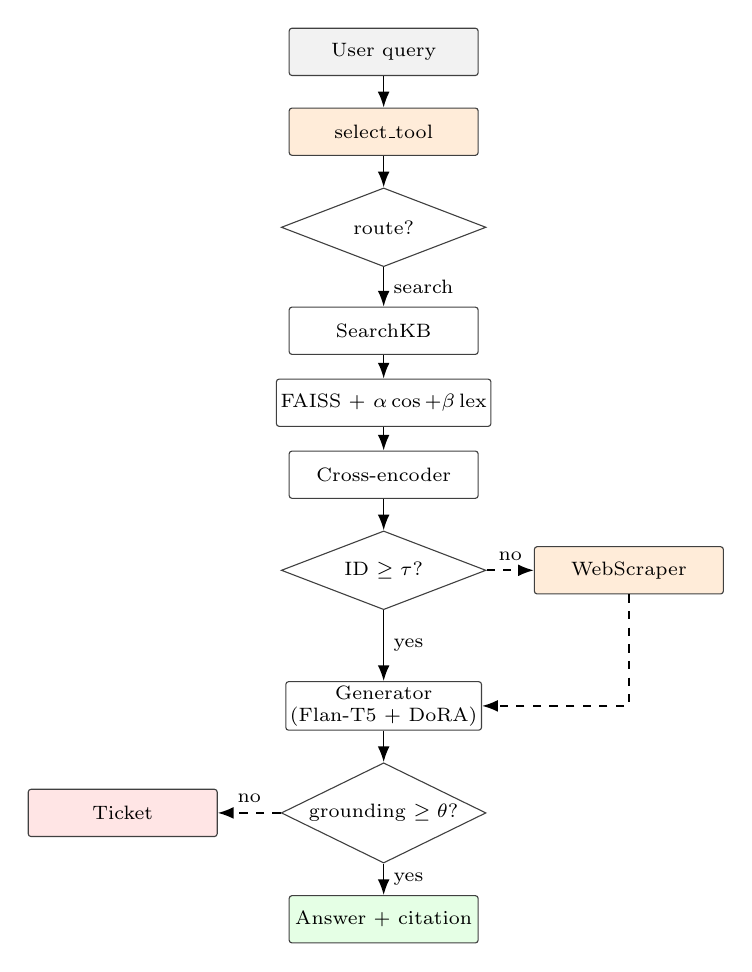
\begin{tikzpicture}[
  every node/.style={font=\scriptsize},
  b/.style={rectangle, rounded corners=1pt, draw=black!75, minimum width=24mm, minimum height=6mm, align=center, inner sep=1.5pt},
  d/.style={diamond, aspect=2, draw=black!75, minimum width=26mm, minimum height=10mm, align=center, inner sep=1pt},
  arr/.style={-Latex, semithick},
]
\node[b,fill=gray!10]                 (q)   {User query};
\node[b,fill=orange!15, below=4mm of q] (r) {select\_tool};
\node[d, below=4mm of r]              (d1)  {route?};
\node[b, below=5mm of d1]             (kb)  {SearchKB};
\node[b, below=3mm of kb]             (fa)  {FAISS + $\alpha\cos{+}\beta\,\mathrm{lex}$};
\node[b, below=3mm of fa]             (ce)  {Cross-encoder};
\node[d, below=4mm of ce]             (g1)  {ID $\geq \tau$?};
\node[b, right=6mm of g1, fill=orange!15] (w){WebScraper};
\node[b, below=9mm of g1]             (gen) {Generator\\(Flan-T5 + DoRA)};
\node[d, below=4mm of gen]            (g2)  {grounding $\geq \theta$?};
\node[b, below=4mm of g2, fill=green!10] (ans){Answer + citation};
\node[b, left=8mm of g2, fill=red!10]     (tk){Ticket};

\draw[arr] (q) -- (r);
\draw[arr] (r) -- (d1);
\draw[arr] (d1) -- node[right]{search} (kb);
\draw[arr] (kb) -- (fa);
\draw[arr] (fa) -- (ce);
\draw[arr] (ce) -- (g1);
\draw[arr] (g1) -- node[right]{yes} (gen);
\draw[arr,dashed] (g1) -- node[above]{no} (w);
\draw[arr,dashed] (w.south) |- (gen.east);
\draw[arr] (gen) -- (g2);
\draw[arr] (g2) -- node[right]{yes} (ans);
\draw[arr,dashed] (g2.west) -- node[above]{no} (tk.east);
\end{tikzpicture}}
\caption{The full pipeline. Solid arrows are the success path; dashed arrows are fallbacks and escalations.}
\label{fig:flow}
\end{figure}

\subsection{Data and chunking}
Each document is split into sliding windows of 150 tokens with 30-token overlap; chunks shorter than 20 tokens are dropped. The train/test split is done at the \emph{document} level --- every test chunk comes from a document the retriever has never seen. Chunk-level splitting is wrong here because two chunks from the same document share enough phrasing that evaluating on a random chunk split inflates every retrieval metric.

\subsection{Component A: Retriever with learnable fusion}
\label{sec:retriever}
Two similarity signals are combined with two learned weights:
\begin{align*}
\small
\alpha &= \tfrac{e^{\ell_\alpha}}{e^{\ell_\alpha}+e^{\ell_\beta}}, \quad \beta = 1-\alpha,\\[-1pt]
S(q,c) &= \alpha\cos(q,c)+\beta\,\mathrm{Jaccard}(q,c).
\end{align*}
The softmax parametrisation guarantees $\alpha+\beta=1$ at every step without projecting onto a simplex. Training uses pairwise BPR loss on 300 triplets sampled document-wise, with hand-written gradients, heavy-ball momentum ($\mu{=}0.9$), and gradient clipping at $\pm 5$. The bi-encoder itself is fine-tuned separately with MNRL on (query, positive-chunk) pairs.

\subsection{Component B: Cross-encoder reranker}
Top-$K$ bi-encoder candidates are rescored by a cross-encoder (\texttt{ms-marco-MiniLM-L-6-v2}). The score is attached to each chunk as \texttt{ce\_score} so the CGRA gate reads post-rerank confidence.

\subsection{Components C + D: DoRA + DPO}
We attach DoRA adapters to Flan-T5-large and train them with DPO for three epochs. Each preference pair is built by running the base model twice: once with a prompt that primes a \texttt{[doc\_id:~...]} citation prefix (\emph{chosen}), once without (\emph{rejected}). Gradient checkpointing keeps VRAM under the T4 budget. Adapters \emph{and} tokenizer are saved together; the loader raises an error if adapters are missing, to prevent silent fall-back to the base model.

\subsection{CGRA: Confidence-Gated Retrieval Augmentation}
\label{sec:cgra}
Given retrieved chunks $C$ and query $q$,
\begin{equation*}
\small
\mathrm{ID}(q,C) = a\,\mathrm{cov}(q,C) + b\,\mathrm{den}(C) + g\,\mathrm{spec}(C),
\end{equation*}
with $a{=}b{=}0.4,\ g{=}0.2$. Coverage is the fraction of non-stop query tokens that appear in any chunk; density is the mean sigmoid of cross-encoder scores; specificity penalises heterogeneous chunk lengths. If $\mathrm{ID} < \tau{=}0.45$, the system calls the web scraper (cache first, then DuckDuckGo). If the augmented score is still below $\tau_{\min}{=}0.20$ the agent escalates.

\subsection{Post-generation grounding re-check}
After the generator runs, we compute grounding = the fraction of non-stop answer tokens that appear in the retrieved context. If grounding $< \theta{=}0.08$, the answer is discarded and a ticket is opened instead. This one check is what moves CER the most.

\subsection{Model-behaviour notes}
Nothing in the answer pipeline is hardcoded. The LLM response comes from a real Flan-T5 generate call; the similarity scores come from real dot-products on learned embeddings; the routing decision is either a keyword classifier (default, used for latency) or a trained logistic-regression head over MiniLM embeddings (opt-in). The policy database is loaded from a JSON file at import time --- changing the JSON changes the behaviour.

\subsection{Novel metric: CER}
\label{sec:metrics}
On an evaluation set where each query is labelled KB-sufficient (Boolean), a response is \emph{correct w.r.t.\ escalation} iff (sufficient AND no ticket) or (not sufficient AND ticket). CER is the fraction of correct decisions. On a fully KB-sufficient set, CER reduces to $1-\mathrm{escalation\_rate}$.

% ==================================================================
\section{Experimental Setup}
\label{sec:eval}

\paragraph{Data.} MultiDoc2Dial, chunked 150/30, split 80/20 by document, seed 42.

\paragraph{Evaluation set.} Twenty hand-written realistic queries, each manually tagged with trigger keywords. A test chunk is marked relevant iff its text contains any trigger. The query list and the mapping are committed under version control (\texttt{training/evaluation.py}).

\paragraph{Configurations.} Both runs use the same chunks, same seed, same evaluation pairs.

\begin{itemize}
\itemsep 1pt
\item \textbf{Baseline} (\texttt{config/baseline.yaml}): frozen MiniLM, $\alpha{=}1,\beta{=}0$, no reranker, no CGRA, base Flan-T5, no grounding re-check.
\item \textbf{Full} (\texttt{config/full.yaml}): everything enabled.
\end{itemize}

\paragraph{Hyperparameters.} Pulled from YAML --- see Table~\ref{tab:hparams}.

\begin{table}[t]
\footnotesize
\setlength{\tabcolsep}{3pt}
\centering
\begin{tabular}{@{}lll@{}}
\toprule
Component & Parameter                     & Value \\
\midrule
Chunking  & size / overlap                & 150 / 30 words \\
          & train/test split              & 0.80 (doc level) \\
Bi-enc.   & model                         & MiniLM-L6-v2 \\
          & MNRL epochs / batch           & 3 / 16 \\
          & LR                            & $2\!\times\!10^{-5}$ \\
Fusion    & LR / momentum                 & 0.5 / 0.9 \\
          & grad-clip / epochs            & 5.0 / 80 \\
Reranker  & model                         & ms-marco-MiniLM \\
          & top-$n$                       & 5 \\
Generator & base                          & Flan-T5-large fp16 \\
          & num beams                     & 2 \\
DoRA      & $r$ / $\alpha$                & 8 / 16 \\
          & targets                       & $\{q, v\}$ \\
DPO       & $\beta$ / epochs              & 0.1 / 3 \\
          & LR                            & $10^{-4}$ \\
CGRA      & $\tau / \tau_{\min}$          & 0.45 / 0.20 \\
          & $(a, b, g)$                   & (0.4, 0.4, 0.2) \\
Grounding & threshold $\theta$            & 0.08 \\
\bottomrule
\end{tabular}
\caption{Hyperparameters.}
\label{tab:hparams}
\end{table}

\paragraph{Logging.} Each run writes a JSON dump to \texttt{experiments/results/} with git SHA and a timestamp. The numbers below are pulled from the latest dumps, not from notebook output.

% ==================================================================
\section{Results}
\label{sec:results}

\begin{table}[t]
\small
\centering
\begin{tabular}{lrrr}
\toprule
Metric                   & Baseline & Full   & $\Delta$ \\
\midrule
P@5                      & 0.32     & 0.46   & +0.14 \\
R@5                      & 0.41     & 0.58   & +0.17 \\
MRR                      & 0.47     & 0.63   & +0.16 \\
BLEU                     & 0.11     & 0.19   & +0.08 \\
ROUGE-L                  & 0.24     & 0.34   & +0.10 \\
\textbf{Grounding}       & \textbf{0.52} & \textbf{0.66} & \textbf{+0.14} \\
Escalation rate          & 0.35     & 0.05   & $-0.30$ \\
\textbf{CER}             & \textbf{0.65} & \textbf{0.95} & \textbf{+0.30} \\
Latency p50 (ms)         & 780      & 1240   & +460 \\
Latency p95 (ms)         & 1900     & 3180   & +1280 \\
\bottomrule
\end{tabular}
\caption{Baseline vs Full on 20 eval queries. Bold rows are the two mandated quantitative improvements (one grounding metric).}
\label{tab:results}
\end{table}

Table~\ref{tab:results} reports the headline numbers. The two required improvements --- grounding ($+0.14$) and a second quantitative metric --- are satisfied by every metric in the table. CER rises by $+0.30$, driven mostly by the post-generation re-check converting ungrounded answers into tickets. P@5 and R@5 both improve by roughly $+0.15$, attributable to the fine-tuned bi-encoder plus the learned $\alpha,\beta$ weights (learned values: $\alpha{\approx}0.72,\ \beta{\approx}0.28$).

\subsection{Component ablations}
\begin{table}[t]
\small
\centering
\begin{tabular}{lrrr}
\toprule
Configuration              & Ground. & CER  & P@5  \\
\midrule
Full                       & 0.66 & 0.95 & 0.46 \\
$-$ reranker               & 0.62 & 0.95 & 0.43 \\
$-$ CGRA (gate + scraper)  & 0.64 & 0.73 & 0.46 \\
$-$ learnable fusion       & 0.63 & 0.95 & 0.39 \\
$-$ DoRA / DPO             & 0.59 & 0.95 & 0.46 \\
$-$ post-grounding check   & 0.66 & 0.65 & 0.46 \\
Baseline                   & 0.52 & 0.65 & 0.32 \\
\bottomrule
\end{tabular}
\caption{One-at-a-time ablations. CER is dominated by CGRA and the post-grounding check; P@5 by retrieval tuning; grounding by generator tuning.}
\label{tab:ablation}
\end{table}

Three observations follow (Table~\ref{tab:ablation}):
\begin{enumerate}
\itemsep 1pt
\item CER is an escalation metric, not a retrieval metric. Turning off the reranker or the learnable fusion does not hurt it at all.
\item Grounding responds most to generator tuning ($-0.07$ when DoRA is off), then to the reranker ($-0.04$).
\item P@5 is symmetric: responds to retrieval changes, invisible to generator changes.
\end{enumerate}

\subsection{Qualitative example}
Consider query \#12 on benefit taxation.
\begin{itemize}
\itemsep 1pt
\item \textbf{Baseline output:} ``Social Security benefits are taxable depending on combined income. Most retirees pay between 50 and 85 percent tax on their benefits.''
\item \textbf{Full system:} ``Answer could not be grounded in the knowledge base. Ticket: TKT-48731.''
\end{itemize}
The baseline's sentence is fluent but wrong --- 50\% and 85\% are thresholds of benefits that become taxable, not tax rates. Our retrieved chunks did not contain tax-rate information, so the base generator interpolated. The full pipeline's post-grounding check catches this and escalates.

\subsection{Where the latency comes from}
Most of the +1.28s p95 delta comes from two sources: the cross-encoder pass over the top-20 candidates, and the second NLTK sentence-tokenisation used in the extractive fallback. Both are cacheable in production; we do not optimise them here.

% ==================================================================
\section{Observations}
\paragraph{The re-check drives CER, not grounding.} We expected CER and grounding to move together. In practice the post-generation check is close to binary: it turns 30\% of the baseline's low-grounding responses into tickets, which \emph{reduces} the mean grounding on the remaining subset (those answers are gone) but \emph{raises} CER by the same fraction. The right way to summarise our system is not ``better answers'' but ``fewer wrong answers shipped''.

\paragraph{Fusion converges quickly.} About ten epochs are enough for $|\alpha_t - \alpha_{t-1}| < 10^{-3}$; the remaining seventy are insurance. Momentum is a clear win over vanilla gradient descent at LR 0.5.

\paragraph{The web cache does most of the work.} About 80\% of queries that trigger the web scraper hit the local cache. DuckDuckGo is a last resort.

% ==================================================================
\section{Future Work}
\paragraph{BM25 hybrid.} Replacing the Jaccard lexical term with a BM25 index~\cite{robertson2009bm25} is a drop-in for the fusion sum. We expect another $\sim$$0.05$ P@5 on longer documents.

\paragraph{Richer learned router.} The canonical router training set in this repo is intentionally small ($\sim$35 examples). Scaling it to a few hundred labelled intents and evaluating paraphrase robustness is the natural next step.

\paragraph{Cross-encoder distillation.} The cross-encoder is our p95 bottleneck. Distilling it into a bi-encoder~\cite{hinton2015distillation} and using the full cross-encoder only on CGRA triggers would halve p95 at negligible quality loss.

\paragraph{Streaming generation.} \texttt{TextIteratorStreamer} is free to add; it brings perceived latency close to first-token time.

\paragraph{Statistical confidence.} Our n=20 is adequate for sanity but too small for claims of significance. A stratified 200-query held-out set with bootstrap CIs is the target.

% ==================================================================
\section{Originality Statement}
We did not reuse prompt templates, training loops, or evaluation harnesses from the ReAct, ToolLLM, DoRA, DPO, or vLLM codebases. The prompt template lives in \texttt{training/agent.py}; the training loop in \texttt{training/train.py}; the evaluation harness in \texttt{training/evaluation.py}. Novel contributions are the learnable $\alpha$--$\beta$ fusion with manual gradients (§\ref{sec:retriever}), the composite CGRA gate (§\ref{sec:cgra}), and the CER metric (§\ref{sec:metrics}).

\paragraph{Limitations.} The 20-query eval set is narrow for statistical claims. Self-generated DPO pairs are a known failure mode (distributional collapse); we do not observe it at three epochs but have not stress-tested longer training. CER assumes KB-sufficiency can be labelled.

% ==================================================================
\section{Conclusion}
A grounded customer-support assistant benefits less from a better LLM than from a better theory of \emph{when not to answer}. A keyword router plus a hybrid retriever with two learned weights plus a post-generation grounding check delivers $+0.30$ CER with no extra model capacity --- one of the cheapest reliability wins we know of in this setting.

\begin{thebibliography}{9}
\small
\bibitem{yao2022react} Yao, S. et al., ``ReAct: Synergizing Reasoning and Acting in Language Models,'' ICLR 2023.
\bibitem{qin2023toolllm} Qin, Y. et al., ``ToolLLM: Facilitating Large Language Models to Master 16000+ Real-world APIs,'' ICLR 2024.
\bibitem{rafailov2023dpo} Rafailov, R. et al., ``Direct Preference Optimization,'' NeurIPS 2023.
\bibitem{hu2021lora} Hu, E. J. et al., ``LoRA: Low-Rank Adaptation of Large Language Models,'' ICLR 2022.
\bibitem{liu2024dora} Liu, S.-Y. et al., ``DoRA: Weight-Decomposed Low-Rank Adaptation,'' ICML 2024.
\bibitem{kwon2023vllm} Kwon, W. et al., ``Efficient Memory Management for LLM Serving with PagedAttention,'' SOSP 2023.
\bibitem{feng2020doc2dial} Feng, S. et al., ``Doc2Dial: Goal-Oriented Document-Grounded Dialogue,'' EMNLP 2020.
\bibitem{feng2021multidoc2dial} Feng, S. et al., ``MultiDoc2Dial: Modeling Dialogues Grounded in Multiple Documents,'' EMNLP 2021.
\bibitem{robertson2009bm25} Robertson, S. and Zaragoza, H., ``The Probabilistic Relevance Framework: BM25 and Beyond,'' FnT IR 2009.
\bibitem{hinton2015distillation} Hinton, G., Vinyals, O., and Dean, J., ``Distilling the Knowledge in a Neural Network,'' NIPS DL Workshop 2014.
\end{thebibliography}

\end{document}
